\chapter{Исследование устойчивости системы квантовой коммуникации на боковых частотах к атакам на измерительное оборудование}  \label{ch:ch2}


\section{Детектор в составе системы} \label{sec:ch2/sec1}

В зависимости от поставленных целей и решаемых задач в состав систем квантовой коммуникации включают в основном два типа детекторов одиночных фотонов, сравнительная характеристика которых дана в главе \ref{sec:ch1/sec5}. Для магистральных дистанций от 100~км, либо для обеспечения высокой скорости формирования квантовых кодирующих последовательностей применяют сверхпроводниковые ДОФ (SNSPD). Для внутригородских дистанций до 100~км с потерями в линиях связи менее 15~дБ обычно применяют более компактный, простой в использовании ДОФ на базе лавинного фотодиода (SPAD), однако его типовые характеристики на порядок уступают характеристикам сверхпроводникового ДОФ. 


В СКК на боковых частотах применяется коммерчески доступный детектор модели ID210, разработанный компанией idQuantique. Его отличительными особенностями являются:
\begin{enumerate}
	\item Поддержка высокой частоты стробирующих импульсов - до 100~МГц
	\item Возможность подачи стробирующих импульсов от внешнего устройства (External gating mode)
	\item Широкий диапазон настройки ширины окна срабатывания (gate) - от 0,5~нс до 25~нс
	\item Выставление задержки открытия окна срабатывания относительно стробирующего импульса (Trigger delay) в диапазоне до 10~нс с высоким разрешением во времени - 10~пс 
	\item Возможность выставления <<мертвого времени>> в широком диапазоне - от 0,1~мкс до 100~мкс
	\item Возможность регулировки квантовой эффективности с шагом 2,5~\% в диапазоне от 5~\% до 25~\%
	\item Полупроводниковая структура ЛФД - InGaAs/InP
	\item Относительно низкий уровень темнового счета при заданных параметрах квантовой эффективности
\end{enumerate}


В ходе исследования для обеспечения реалистичных условий атаки злоумышленника на измерительное оборудование в составе СКК устройство рассматривалось, как <<черный ящик>>, то есть оно не вскрывалось и не производились манипуляции с внутренними платами и микросхемами. Все настройки детектора выставлялись в соответствии со штатным режимом для систем квантовой коммуникации на боковых частотах модулированного излучения. Основные настройки вынесены в таблицу \ref{tab:ID210_setups}.  




\begin{table} 
	\centering
	\caption{Типовые настройки детектора ID210 в составе СКК}
	\label{tab:ID210_setups}
		\begin{tabular}{|c|c|c|}
			\hline
				№  				& Параметр    				 & Значение     \\
			\hline
				1 				& Квантовая эффективность,~\% 	 & 10 		 \\
			\hline 

				2 				& Частота стробирования,~Гц 		 & $10^8$   \\
			\hline

				3 				& Ширина окна,~нс & 5 	     \\
			\hline

				4 				& <<Мертвое>> время,~нс  & 100 		  \\
			\hline

				5 				& Частота темновых срабатываний,~Гц & 200 		  \\

			\hline
		\end{tabular}
\end{table}




%%%%%%%%%%%%%%%%%%%%%%%%%%%%%%%%%%%%%%%%%%%%%%%%%%%%%%%%%%%%%%%%%%%%%%%%%%%%%%%%%%%%%%%%%%%%%%%%%%%%%%%%%%%%%%%%%

\section{Выведение детектора из режима Гейгера} \label{sec:ch2/sec2}

Первым этапом проведения атаки с навязыванием ключа является определение возможности выведения детектора из режима счета фотонов (режима Гейгера). Известно, что вольт-амперная характеристика лавинного фотодиода имеет вид, представленный на рисунке \ref{fig:APDs_VA}.    

 \begin{figure}[ht]
  \centering
  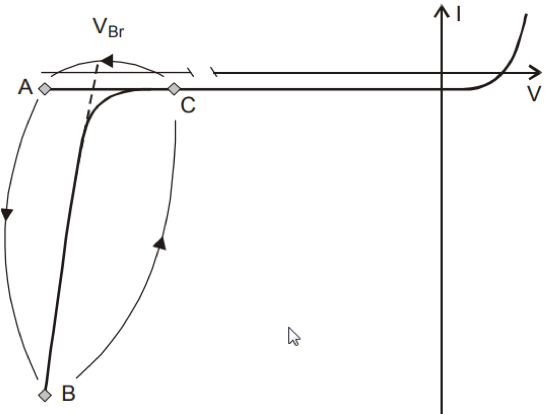
\includegraphics{APDs_VA.png}
  \caption{Вольт-амперная характеристика ЛФД}
  \label{fig:APDs_VA}
\end{figure}


Лавинный фотодиод работает при обратном напряжении смещения $-V_{bias}$ близком к напряжению пробоя $-V_{breakdown}$. Типичная величина находится в диапазоне от -40~В до -60~В. При величине обратного напряжения смещения ниже напряжения пробоя ЛФД находится в линейном режиме, где величина фототок $I_{APD}$ линейно зависит от падающей оптической мощности. При увеличении величины обратного смещения выше напряжения пробоя ЛФД переходит в режим счета фотонов, или режим Гейгера. В этом режиме даже энергии единиц фотонов достаточно для формирования лавины зарядов и резкого скачка фототока. При превышении некоторого порогового значения $I_{det}$, регулируемого уровнем срабатывания компаратора, формируется электрический импульс, который и интерпретируется, как регистрация одиночного фотона. 

 \begin{figure}[ht]
  \centering
  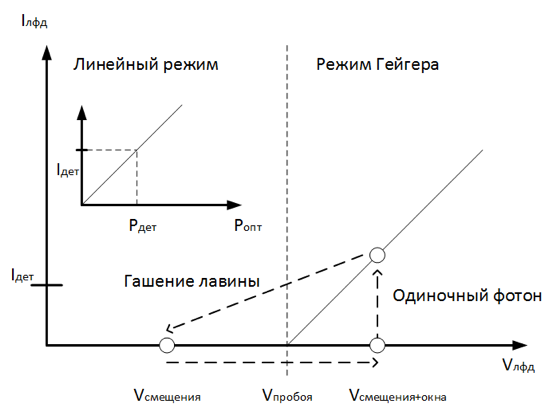
\includegraphics{Vbreakdown}
  \caption{Граница между режимами работы ЛФД при подаче обратного напряжения смещения}
  \label{fig:Vbreakdown}
\end{figure}

Гашение лавины в самом простом случае происходит благодаря последовательно подключенному в цепь резистору, как показано на рисунке \ref{fig:Quenching}. Существуют также схемы активного гашения лавины.  
 \begin{figure}[ht]
  \centering
  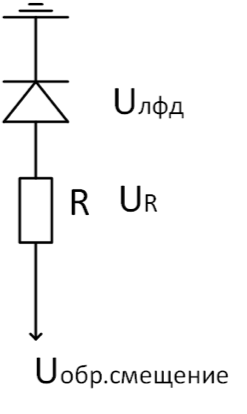
\includegraphics{Quenching}
  \caption{Принципиальная электрическая схема подключения ЛФД для регистрации одиночных фотонов}
  \label{fig:Quenching}
\end{figure}


Для снижения уровня шумов срабатываний ДОФ на базе ЛФД функционируют в режиме стробирования, когда в момент ожидаемого прибытия фотона на диод подается дополнительное напряжение в форме импульса, т.\:н. окно срабатывания $-V_{gate}$, величиной около 3~В. Благодаря этому импульсу диод переходит из линейного режима при величине напряжении $-V_{bias}$, в котором он прибывает относительно длительное время порядка единиц микросекунд, в режим счета фотонов, где $-V_{bias+gate} < - V_{breakdown}$.  

%%%%%%%%%%%%%%%%%%%%%%%%%%%%%%%%%%%%%%%%%%%%%%%%%%%%%%%%%%%%%%%%%%%%%%%%%%%%%%%%%%%%%%%%%%%%%%%%%%%%%%%%%%%%%%%%%

\section{Оптическая схема выведения детектора из режима Гейгера} \label{sec:ch2/sec3}

Для успешного осуществления атаки с навязыванием ключа злоумышленнику требуется манипулировать детектором, то есть форсировать срабатывания и их отсутствие в нужные моменты времени, при этом предполагается, что тип применяемого измерительного оборудования известен, но непосредственный доступ к нему отсутствует. В таких рамках модель атаки ограничивается возможностью воздействия на детектор только оптическими методами непосредственно из квантового канала. 


Известно, что в линейном режиме работы ЛФД при подачи на него постоянной оптической мощности увеличивается фототок, следовательно при подаче постоянного значения напряжение обратного смещения $-V_{bias}$ и при наличии в цепи гасящего лавину резистора, величина падения напряжения на резисторе растет, а на ЛФД снижается (рис.\ref{fig:Quenching}. Суть атаки с выведением детектора из режима Гейгера, или <<ослеплением>> ДОФ, сводится к тому, чтобы сместить режим работы относительно напряжения пробоя ЛФД. При таком подходе даже дополнительных импульсов $V_{gate}$ становится недостаточно и диод все время находится в режиме линейной зависимости фототока от величины мощности оптического излучения, падаюшего на него.  

Тем не менее, как указано на рисунке \ref{fig:Vbreakdown}, в линейном режиме остается возможность превысить пороговое значение фототока $I_{det}$ и сформировать импульс срабатывания детектора.

Таким образом, методика выведения детектора из режима счета фотонов в линейный режим для осуществления атаки с навязыванием ключа (\todo{<<Faked-state attack>>}) легко формализуется. Экспериментальное исследование уязвимости детектора одиночных фотонов к такому типа атак реализуется в три этапа, представленных на рисунке \ref{fig:Method_2.3}:

 \begin{enumerate}
	\item Определение величины постоянной оптической мощности, достаточной для выведения детектора из режима Гейгера
	\item Подстройка оптического импульса под окно срабатывания детектора одиночных фотонов
	\item Определение зависимости вероятности срабатывания детектора от величины энергии фотонов в импульсе
\end{enumerate}

 \begin{figure}[ht] 
  \centering
  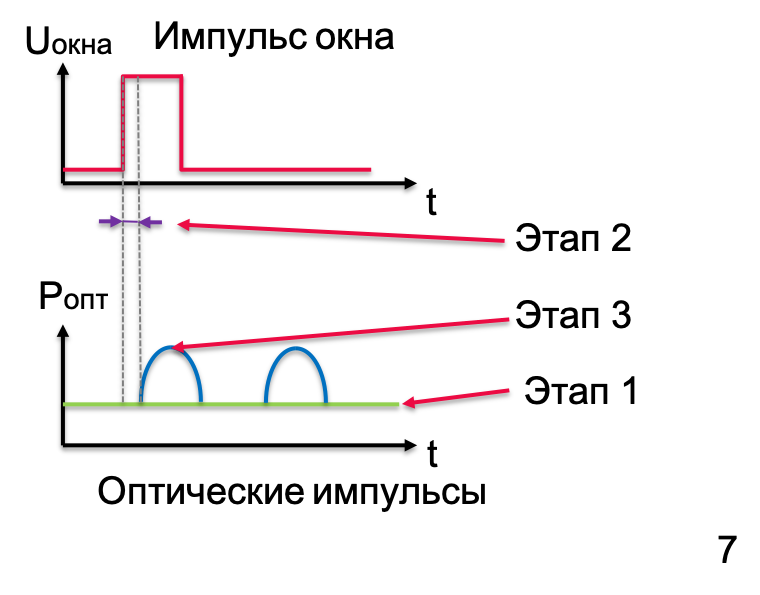
\includegraphics{Method_2.3.eps}
  \caption{Методика выведения детектора из режима Гейгера}
  \label{fig:Method_2.3}
\end{figure}

%
%  На рисунке \ref{fig:Scheme_2.3} представлена принципиальная оптическая схема для проведения исследования уязвимости детектора. 
%
% \begin{figure}[ht] 
%  \centering
%  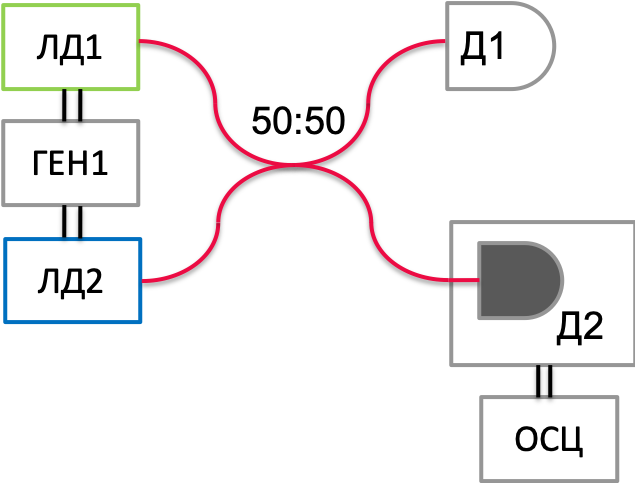
\includegraphics{Scheme_2.3.eps}
%  \caption{Принципиальная оптическая схема эксперимента}
%  \label{fig:Scheme_2.3}
% \end{figure}

%%%%%%%%%%%%%%%%%%%%%%%%%%%%%%%%%%%%%%%%%%%%%%%%%%%%%%%%%%%%%%%%%%%%%%%%%%%%%%%%%%%%%%%%%%%%%%%%%%%%%%%%%%%%%%%%%

\section{Корреляция оптической мощности в плечах светоделителя} \label{sec:ch2/sec4}


Для того, чтобы одновременно производить воздействие оптическим излучением на исследуемый детектор одиночных фотонов и фиксировать величину этого воздействия в оптической схеме используется светоделитель 2х2 с коэффициентом деления 50:50. Один выход подключен к детектору (Д2), второй к измерителю оптической мощности (Д1), как показано на рисунке \ref{fig:Scheme_2.4}. Однако, обычно в волоконно-оптических элементах наблюдается небольшое отклонение основных величин, характеризующих устройство, от паспортных значений. Для того, чтобы скорректировать это отклонение, при помощи двух измерителей оптической мощности фиксируется величина оптической мощности на обоих выходах светоделителя и находится разница между двумя величинами в зависимости от напряжения, подаваемого с генератора (ГЕН1) на лазерный диод (ЛД1), применяемый для выведения детектора и режима Гейгера.   

 \begin{figure}[ht]
  \centering
  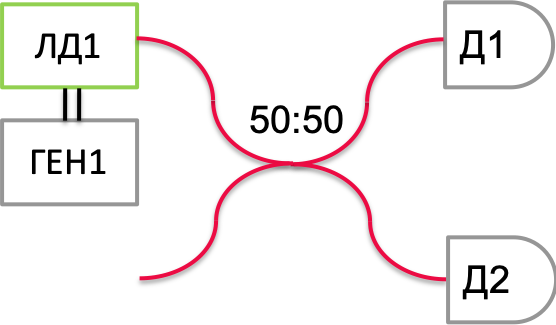
\includegraphics{Scheme_2.4.eps}
  \caption{Принципиальная оптическая схема эксперимента}
  \label{fig:Scheme_2.4}
\end{figure}


График зависимости представлен на рисунке \ref{fig:Beamsplitter}. Видно, что расхождение оставляет величину не превышающую 1 дБ. Соответственно, далее при проведении всех измерений производится корректировка на полученную величину. Таким образом учитывается неидеальность коэффициента деления используемого волоконно-оптического светоделителя 2х2. 


 \begin{figure}[ht]
  \centering
  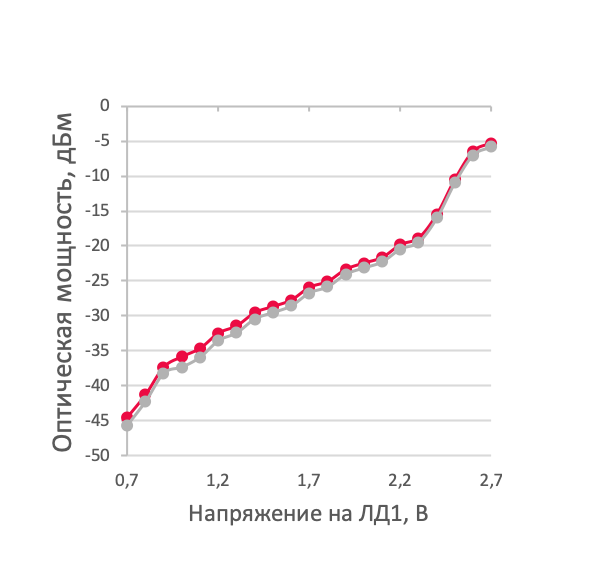
\includegraphics{Beamsplitter.png}
  \caption{Зависимость оптической мощности на двух выходах светоделителя 2х2 от величины напряжения на ЛД1}
  \label{fig:Beamsplitter}
\end{figure}
\pagebreak

%%%%%%%%%%%%%%%%%%%%%%%%%%%%%%%%%%%%%%%%%%%%%%%%%%%%%%%%%%%%%%%%%%%%%%%%%%%%%%%%%%%%%%%%%%%%%%%%%%%%%%%%%%%%%%%%%

\section{Определение величины постоянной оптической мощности, достаточной для выведения детектора из режима Гейгера} \label{sec:ch2/sec5}

На первом этапе выведения детектора из режима счета фотонов требуется определить необходимую и достаточную величину оптической мощности для <<ослепления>> детектора. Характерной особенностью и показателем успешного завершения первого этапа является отсутствие темновых срабатываний ДОФ в линейном режиме. Таким образом, задача сводится к тому, чтобы направить в детектор оптическое излучения в области спектральной чувствительности детектора, для простоты имитации действий злоумышленника это будет длина волны 1550~нм, и зафиксировать смену растущего количества отсчетов их полным отсутствием. На рисунке \ref{fig:Scheme_2.5} представлена оптическая схема эксперимента. 


 \begin{figure}[ht]
  \centering
  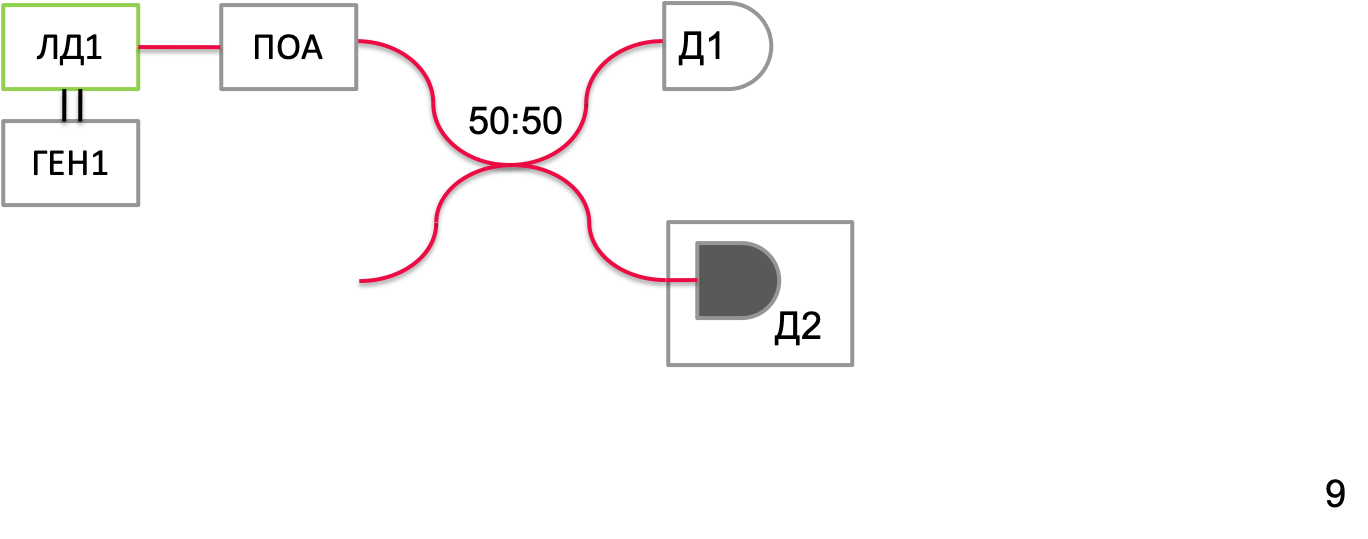
\includegraphics{Scheme_2.5.eps}
  \caption{Принципиальная оптическая схема эксперимента}
  \label{fig:Scheme_2.5}
\end{figure}

В качестве источника постоянного излучения применяется лазерный модуль с распределенной обратной связью (Alcatel 1905 LMI). Излучаемая длина волны - 1550~нм. Особенностями данного модуля так же являются узкая спектральная полоса порядка 2~МГц и встроенный оптический изолятор, предотвращающий попадание переотраженного излучения обратно в лазерный диод. 
 На лицевой панели индикатор количества отсчетов показывает все нули. 



%%%%%%%%%%%%%%%%%%%%%%%%%%%%%%%%%%%%%%%%%%%%%%%%%%%%%%%%%%%%%%%%%%%%%%%%%%%%%%%%%%%%%%%%%%%%%%%%%%%%%%%%%%%%%%%%%




\section{Подстройка оптического импульса под окно детектора одиночных фотонов} \label{sec:ch2/sec6}


 \begin{figure}[ht]
  \centering
  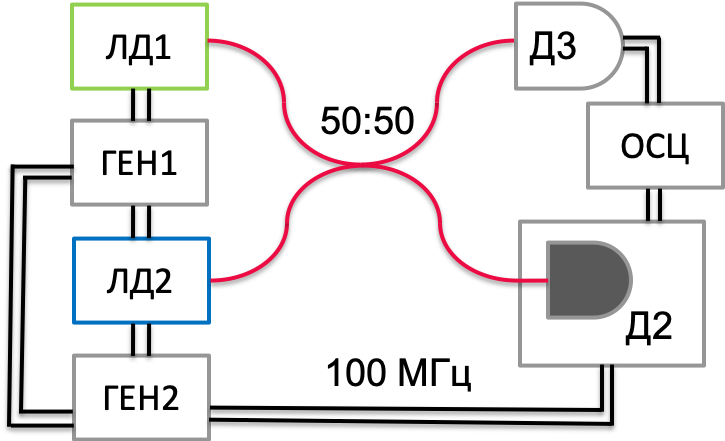
\includegraphics{Scheme_2.6.eps}
  \caption{Принципиальная оптическая схема эксперимента}
  \label{fig:Scheme_2.6}
\end{figure}

%%%%%%%%%%%%%%%%%%%%%%%%%%%%%%%%%%%%%%%%%%%%%%%%%%%%%%%%%%%%%%%%%%%%%%%%%%%%%%%%%%%%%%%%%%%%%%%%%%%%%%%%%%%%%%%%%


\section{Определение количества срабатываний детектора от величины мощности оптического излучения} \label{sec:ch2/sec7}


 \begin{figure}[ht]
  \centering
  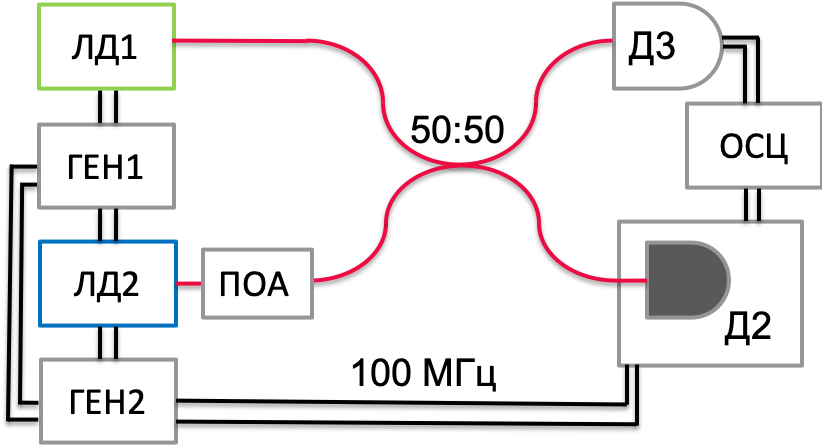
\includegraphics{Scheme_2.7.eps}
  \caption{Принципиальная оптическая схема эксперимента}
  \label{fig:Scheme_2.7}
\end{figure}



%%%%%%%%%%%%%%%%%%%%%%%%%%%%%%%%%%%%%%%%%%%%%%%%%%%%%%%%%%%%%%%%%%%%%%%%%%%%%%%%%%%%%%%%%%%%%%%%%%%%%%%%%%%%%%%%%


\section{Определение зависимости вероятности срабатывания детектора от величины мощности оптического излучения в квантовом канале} \label{sec:ch2/sec8}




%%%%%%%%%%%%%%%%%%%%%%%%%%%%%%%%%%%%%%%%%%%%%%%%%%%%%%%%%%%%%%%%%%%%%%%%%%%%%%%%%%%%%%%%%%%%%%%%%%%%%%%%%%%%%%%%%


\section{Определение зависимости вероятности срабатывания детектора от величины энергии фотонов в импульсе} \label{sec:ch2/sec9}


%%%%%%%%%%%%%%%%%%%%%%%%%%%%%%%%%%%%%%%%%%%%%%%%%%%%%%%%%%%%%%%%%%%%%%%%%%%%%%%%%%%%%%%%%%%%%%%%%%%%%%%%%%%%%%%%%
\section{Атака с навязыванием ключа «поддельными» состояниями} \label{sec:ch2/sec10}


%%%%%%%%%%%%%%%%%%%%%%%%%%%%%%%%%%%%%%%%%%%%%%%%%%%%%%%%%%%%%%%%%%%%%%%%%%%%%%%%%%%%%%%%%%%%%%%%%%%%%%%%%%%%%%%%%
\section{Границы применимости атаки с навязыванием ключа} \label{sec:ch2/sec11}




%%%%%%%%%%%%%%%%%%%%%%%%%%%%%%%%%%%%%%%%%%%%%%%%%%%%%%%%%%%%%%%%%%%%%%%%%%%%%%%%%%%%%%%%%%%%%%%%%%%%%%%%%%%%%%%%%
\section{Оценка возможностей злоумышленника при атаке с выведением детектора из режима Гейгера для систем квантовой коммуникации на боковых частотах} \label{sec:ch2/sec12}



%%%%%%%%%%%%%%%%%%%%%%%%%%%%%%%%%%%%%%%%%%%%%%%%%%%%%%%%%%%%%%%%%%%%%%%%%%%%%%%%%%%%%%%%%%%%%%%%%%%%%%%%%%%%%%%%%
\section{Выводы по главе} \label{ch:ch2/sect13}
